\begin{figure}[h]
\centering
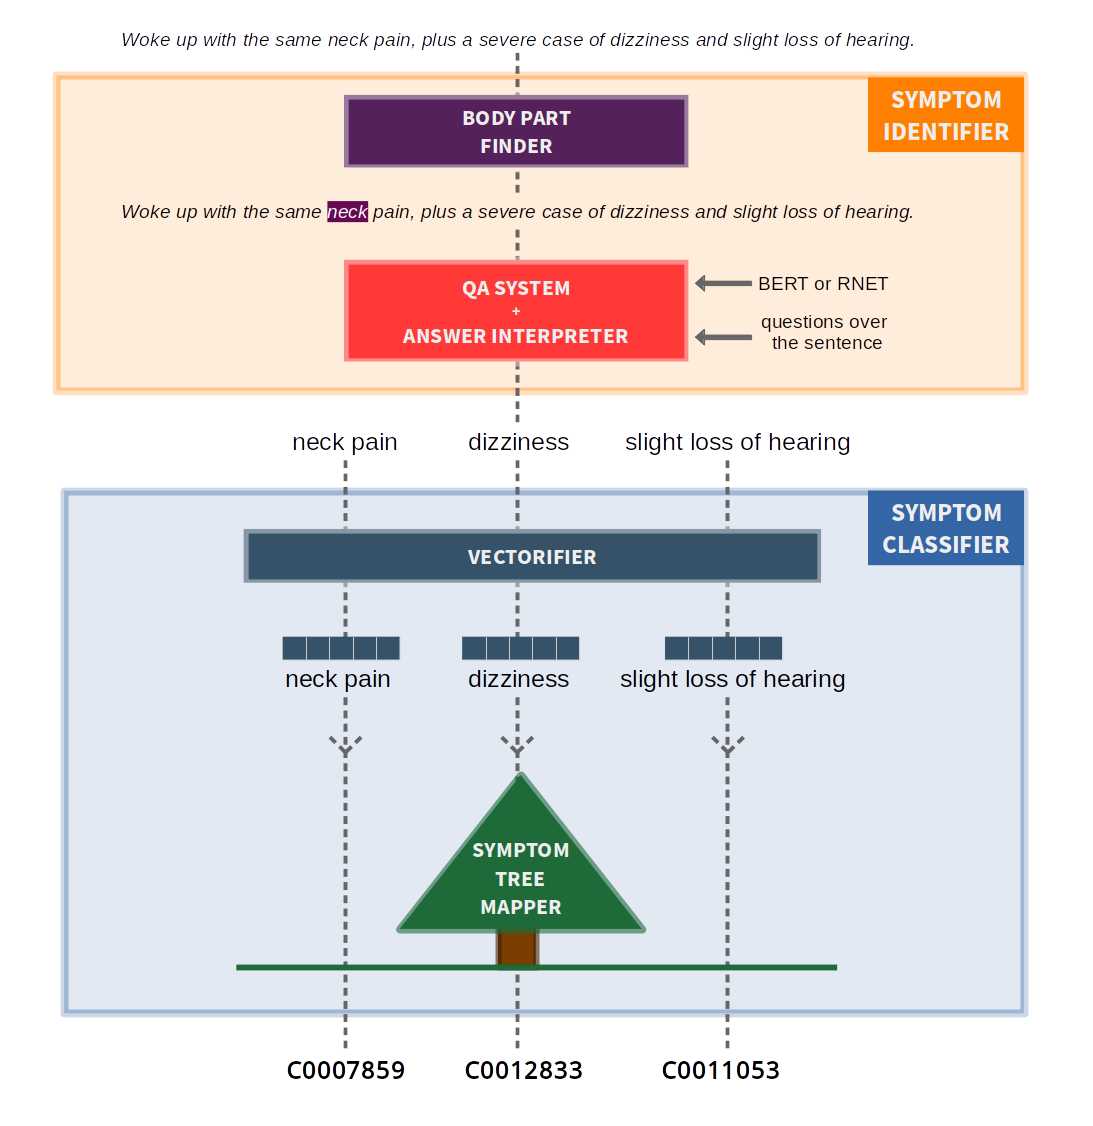
\includegraphics[width=17cm]{methods_overview}
\caption{Overview of methods}
\medskip
\end{figure}

\newpage
\chapter{Methods}
\label{cha:methods}
In this chapter, firstly, the Natural Language Processing methods used in this work are described in detail. Secondly, the aforementioned sub-components are analyzed.

\section{The \textit{Body Part Finder}}
\label{sec:body_part_finder}
\subsection{The body part list}
The objective of this component is to identify body parts words within the patient's sentence. For this goal, it is necessary to have a list of body parts. In addition, each body part can be expressed by the patient using a large variety of terms: its synonyms. Hence, with the addition of an abstraction layer, the list of body parts becomes a list of body parts concepts. Each body part concept is then associated to a list of its synonyms. 

Another problem to face is that the language of the body parts classification should be understandable by every patient: therefore, it has to be informal and not strictly technical.

At the moment, it is not available any body part classification with these features. Therefore, a new classification based on the list of body parts found in \footnote{https://en.wikipedia.org/wiki/Glossary\_of\_medicine} \cite{bodypartswiki} has been produced by the author. The classification is saved in a \texttt{.csv} file.

\subsection{Finding a body part in a sentence}
Finding a body part in a sentence is trivial if it is available an exhaustive list of body parts and the respective synonyms. The code does a simple string matching between each word in the sentence and each synonym present inside the classification. This approach has some drawbacks: for example, the word “back” can be both a preposition and a body part. Therefore, taking in consideration only words may lead to forget the context: this might introduce misunderstandings, lowering the quality of the results.

\section{Question Answering system}
\label{sec:qa_system}
The outcome of the \textit{Body Part Finder} is then passed to the \textit{QA system}. Its aim is highlighting, in the patient's sentence, the words that answers to a set of questions like \textit{What are the symptoms in the sentence?} or \textit{What is the problem with the neck?}. This task is called in literature \textit{Machine Reading Comprehension} \cite{rnet}.

\subsection{Types of questions}
The questions asked to the specified model over each sentence can be of two types:
\begin{enumerate}
  \item generic question about the symptoms in the sentence: \textit{What are the symptoms?}
  \item specific question about the problem of a found body part in the sentence: \textit{What is the problem with the }\texttt{[body part]}?
\end{enumerate}

The question over the symptoms is intentionally generic because its scope is to catch the majority of the symptoms within the sentence. Thus, as shown in section \ref{sec:answer_interpreter}, the answer to this question must be interpreted.

At the same time, the question over a body part is deliberately specific. The logic behind this question is that if a patient refers to a body part during the interview, can be the source of a problem.

Figure \ref{fig:qa} shows the whole component.

%% IMAGE ABOUT QA SYSTEM
\begin{figure}[h]
\centering
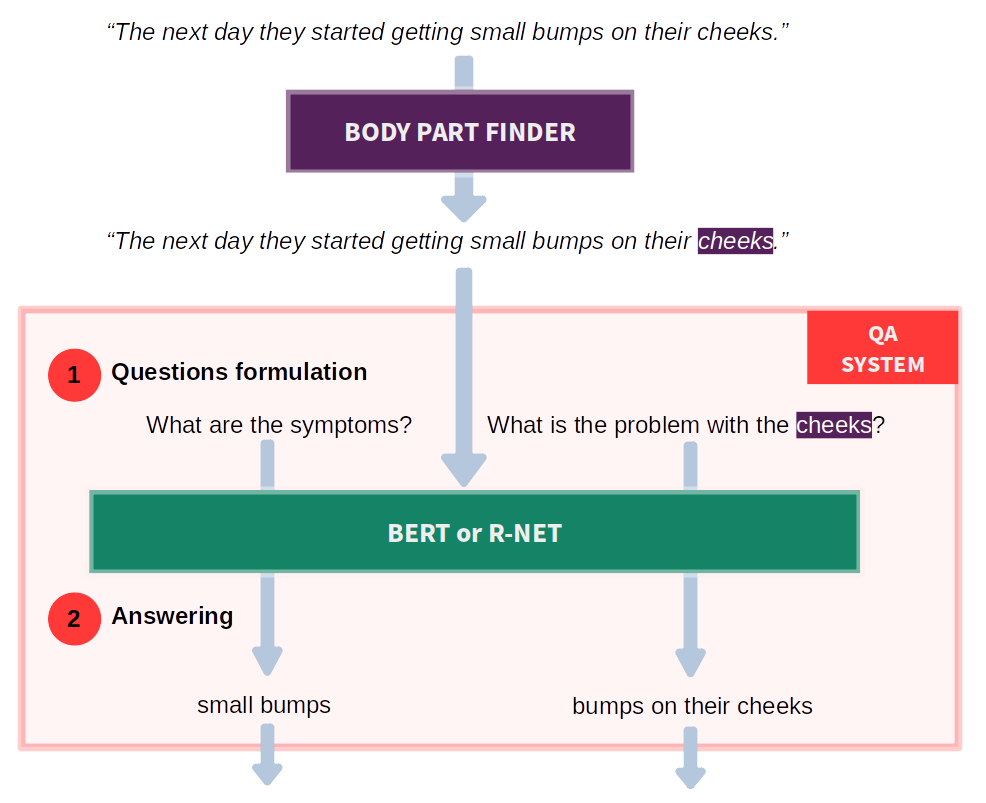
\includegraphics[width=14cm]{qa_sys}
\caption{The \textit{QA system} illustated.}
\medskip
\label{fig:qa}
\end{figure}

As shown in Figure \ref{fig:qa}, two problems may arise: 
\begin{enumerate}
  \item the model can sometimes provide an useful answer but too generic (this is the case of \textit{small bumps})
  \item it might provide redundant answers, increasing unnecessarily the number of predictions.
\end{enumerate}

\subsection{BERT}
Even if I did not personally fine-tuned BERT on SQuAD (I used DeepPavlov's pretrained BERT-SQuAD \cite{deeppavlov}), in this subsection I will briefly outline the characteristics that made BERT a revolutionary model.

BERT, which stands for Bidirectional Encoder Representations from Transformers, is a new language representation model. Even if BERT was presented to the research world in May 2019, it has yet obtained new state-of-the-art results on eleven natural language processing tasks. For instance, a finetuned BERT push SQuAD v1.1 question answering F1 Test to 93.2 (1.5 points of absolute improvement) and SQuAD v2.0 F1 Test to 83.1 (5.1 points of absolute improvement) \cite{bert}.

The training framework proposed by Devlin et al., the authors of BERT, is composed of two steps: \textit{pre-training} and \textit{fine-tuning}. During pre-training BERT is trained over different pre-training tasks. The fine-tuning is only over a single downstream task, in our case, the SQuAD task.

% https://arxiv.org/pdf/1706.03762.pdf
BERT’s  model  architecture is a multi-layer bidirectional Transformer encoder. These last components, that are the building blocks of BERT, are implemented as described in the paper \textit{Attention Is All You Need} by Vaswani et al. \cite{attentionisallyouneed}.

Considering BERT Base, the size taken in consideration for this project (the choice was between Base and Large), the hidden layers (i.e. Transformers encoders) are 12, the hidden size is 768 and the number of self-attention heads is 12.

\begin{figure}[t]
\centering
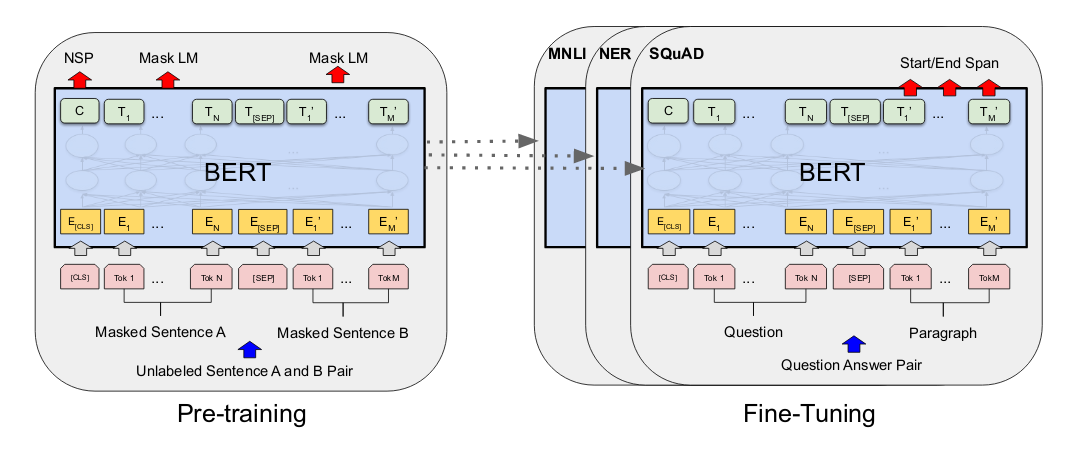
\includegraphics[width=18cm]{bert-for-squad-original-paper}
\caption{Overall pre-training and fine-tuning procedures for BERT. The pre-training procedure provides a basis for the numerous possible downstream tasks. \texttt{[CLS]}, which stands for ``classification'', is a special symbol added in front of every input example, and \texttt{[SEP]} is a special separator token. For further information about the input representation, please read the paper linked in the references. This image is extracted by that paper (\cite{bert}).}
\medskip
\label{fig:bertsquad}
\end{figure}

\subsubsection{Pre-training BERT}
Briefly, pre-training BERT means training it on two tasks:
\begin{itemize}
  \item \textit{Masked Language Model} (MLM), often called \textit{Cloze task}. A bidirectional model like BERT is undoubtedly more powerful than a left-context model like the OpenAI GPT Transformer. But this type of model is even more difficult to train because a bidirectional conditional language model cannot be trained left-to-right or right-to-left, since this would allow each word to indirectly “see itself” during training. Thus, in order to train a bidirectional representation, the researchers simply mask some percentage of the input tokens at random (15\% in their experiments), and then predict those masked tokens. Masking a tokens means substitute a real token with a placeholder token \texttt{[MASK]}. 
  \item \textit{Next Sentence Prediction} (NSP). This task is beneficial to many important downstream tasks like Question Answering and Natural Language Inference that are based on understanding the relation between two sentences, skill that is not captured by the previous task. Basically, this task is a binary \textit{next sentence prediction}: when choosing the sentences \texttt{A} and \texttt{B} for the training, in the 50\% of the cases \texttt{B} is an actual next sentence of \texttt{A} (and it is labeled as \texttt{IsNext}) while in the other cases the choice of \texttt{B} is random between the sentences (labeled as \texttt{NotNext}).
\end{itemize}

% https://arxiv.org/pdf/1606.05250.pdf
\subsubsection{A dataset for Reading Comprehension: SQuAD}
In the fine-tuning stage BERT is trained on SQuAD, a dataset for Reading Comprehension developed by Stanford University \cite{squad}. It consists in a collection of $100\,000$ question-answer pairs over different Wikipedia passages. There are two versions of SQuAD: the first version (\texttt{v1.1}) contains only questions over a passage that have an answer, while the second version (\texttt{v2.0}) have some questions without answer. Obviously, doing better on SQuAD 2.0 is more difficult, because it requires a minimum level of reasoning.

\subsubsection{Fine-tuning BERT on SQuAD1.1}
As illustrated in Figure \ref{fig:bertsquad}, during fine-tuning passage and question are both passed to BERT (separated by the \texttt{[SEP]} tag). This phase introduces two trainable vectors: $S$ (for the start of the answer) and $E$ (for the end of the answer) both of dimension $\mathbb{R}^\mathbb{H}$ ($\mathbb{H}$ is the hidden size, $768$ for BERT Base). 

The probability of a token $i$ of being the start of the answer is $P_{i} = \frac{\mathrm{e}^{S \cdot T_{i}}}{\sum_{j} \mathrm{e}^{S \cdot T_{j}}}$, where $T$ here represents the last layer of BERT. The analogous formula is used for the end of the answer. The score of a candidate span that goes from token $i$ to token $j$ is defined as $score_{i, j} = S \cdot T_{i} + E \cdot T_{j}$. The maximum score where $j \geq i$ is used as prediction. Finally, the training objective is defined as the sum of the two log-likelihoods \eqref{eqn:loglikelihood} of the correct start and end positions.

\begin{equation}
\label{eqn:loglikelihood}
loglikelihood(S) = \sum_{i} y_{i} \mathrm{ln} (P(y_{i} | S)) + (1 - y_{i}) \mathrm{ln} (1 - P(y_{i} | S))
\end{equation}


\subsection{R-NET}
This section will briefly outline R-NET, the other model used for Reading Comprehension. R-NET is trained on SQuAD, dataset described in section \ref{squad}.

R-NET is an end-to-end neural networks model for reading comprehension \cite{rnet}. It performs this task similarly to the way a human does: reading the passage (i.e. the patient's sentence) multiple times. Basically, R-NET tries to improve the passage representation step after step, which are in total three:
\begin{enumerate}
  \item \textit{Question and Passage GRU Layer}. In this layer tokens are converted in GloVe embeddings, and for out-of-vocabulary tokens a character embedding is computed. These vectors are not contextual: for this reason these embeddings are then fed to a BiRNN (composed by Gated Recurrent Units \cite{gru}) in order to ameliorate these representations.
  \item \textit{Question and Passage Matching Layer}. The aim of this layer is to encode the question terms into the passage embeddings of the previous layer. In other words, this permits to the network, given a token in the passage, to focus only on the relevant tokens in the question and tune the passage embeddings to be more similar to the relevant question vectors. This is done using \textit{Attention}.
  
In order to explain this concept, the example taken from \cite{understandingrnet} is reported.

Assuming we are at the highlighted word in the passage:

\begin{displayquote}
She had a talent for \textit{making} home craft tools, mechanical appliances, and the ability to memorize Serbian epic poems.
\end{displayquote}

Given the highlighted token \textit{making}, Attention over the question tokens will highlight the word in italic:

\begin{displayquote}
What were Tesla's mother's special \textit{abilities}?
\end{displayquote}

In this case, \textit{making} embedding is adjusted in order to get it closer to \textit{abilities} embedding. With this procedure, R-NET encodes the question in the passage.

  \item \textit{Passage Self-Matching Layer}. Consider the following passage:
  
  \begin{displayquote}
  Tesla’s mother, Đuka Tesla (née Mandić), whose father was also an Orthodox priest, had a talent for making home craft tools, mechanical appliances, and the \textit{ability} to memorize Serbian epic poems. Đuka had never received a formal education. Nikola credited his eidetic memory and creative \textit{abilities} to his mother’s genetics and influence.
  \end{displayquote}
  
  It is clear that the term \textit{ability} refers to the mother of Tesla, while \textit{abilities} refers to Nikola Tesla. The objective of this step is to capture the difference between terms like those, that, without context, are identical.
  
  Another difficulty resides in \textit{long-term dependencies}: \textit{ability}, for example, is far away from the subject to which the term is referred (Tesla's mother). However, GRU \cite{gru} were developed for addressing the problem of the \textit{vanishing gradients}, which is the reason why vanilla RNNs have troubles with long-term dependencies.
  
  To resolve the former problem, R-NET introduces \textit{Self-Matched Attention}. While with simple Attention a passage term is used to weight a set of vectors (the question terms), with Self-Matched Attention R-NET uses the current passage term to weigh tokens from the passage itself. This helps to make clearer the meaning between ambiguous terms.
\end{enumerate}

Having read and analyzed for three times the passage in the light of the question, the last layer is aimed to output the start and the end of the answer within the passage.

\begin{figure}[t]
% https://slideplayer.com/slide/12351679/
\centering
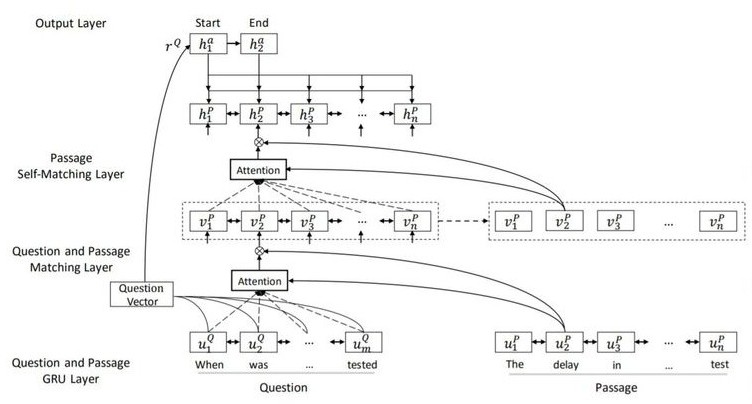
\includegraphics[width=15cm]{rnet}
\caption{A simplified overview of R-NET \cite{imagernetoverview}}
\medskip
\end{figure}



\section{Answer Interpreter}
\label{sec:answer_interpreter}
This component receives the answers of the Question Answering system, interprets them and outputs the \textit{tokens for predictions}.

\subsection{Stemming}
\label{sec:stemming}
Before the interpretation, the answers are stemmed using the \textit{Snowball Stemmer} present in NLTK with a slight modification \cite{snowballstemmer, nltk}. This because it is true that the stemming reduces the variability of text, mapping inflected or derived words into their root form (the stem); but it is also true that a stem does not need to be identical to the morphological word root. This is a problem because a stemmer might output out-of-vocabulary words, which cannot be vectorified. Thus, the solution stands in accepting the stemmed word only if it is inside the vocabulary (the list of the first $100\,000$ terms in GloVe pre-trained embeddings). This stemmer is also used in the calculation of the representative embeddings of symptoms.

\subsection{Filtering ``useless words''}
The stemmed answers are then passed to a function that filters ``useless words''. Basically, it keeps only words that are tagged as a \textit{part of speech} that is inside the following list: noun, adjective, coordinating conjunction, punctuation, verb and auxiliar. For this purpose the Stanford POS Tagger, which is inside Stanford NLP library \cite{stanfordnlp}, was used. Thus, the basic idea is to simplify the answer deleting words like adverbs and pronouns that do not contribute to the meaning of the symptoms.

\subsection{Answer interpretation}
The two different types of answers are processed in a different way:
\begin{itemize}
  \item the general answer about symptoms is one for each passage. Usually, this answer contains more symptoms separated by a coordinating conjunction: mainly, the comma and ``and''. For this reason, the Answer Interpreter splits the answer on these terms and originates one or more \textit{tokens for predictions}.
  \item the specific answers about a body part are as many as the number of body parts found in the passage. Given a body-part answer, the \textit{token for prediction} is formed concatenating the answer with the name of the body part.
\end{itemize}

\begin{figure}[h]
\centering
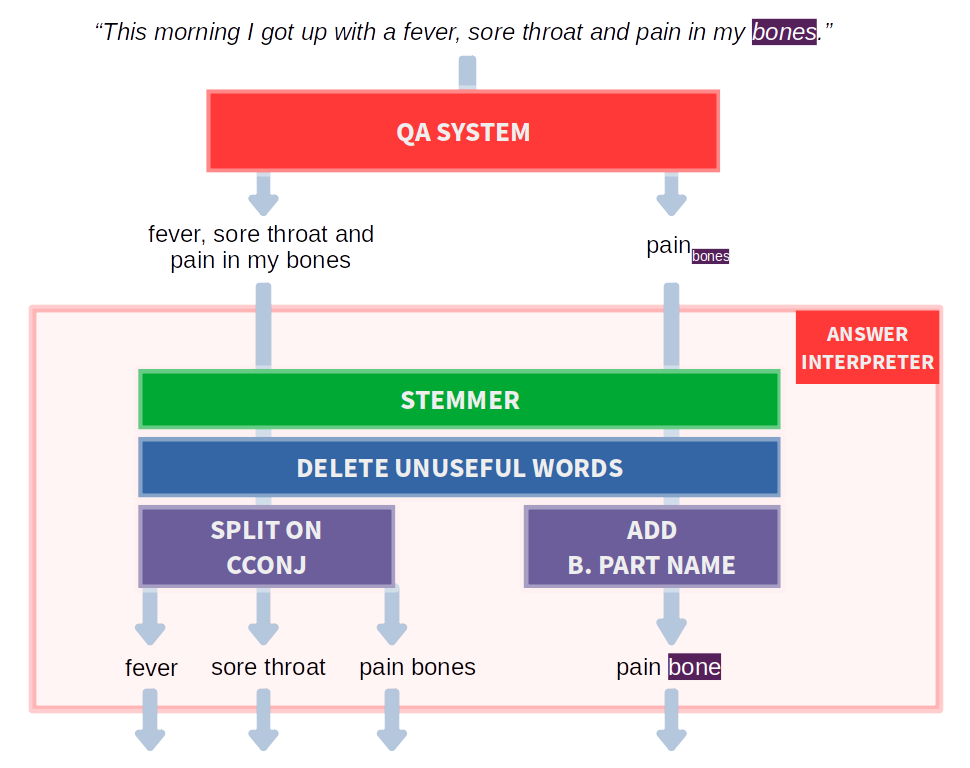
\includegraphics[width=13cm]{answer_interpreter}
\caption{The Answer Interpreter illustrated.}
\medskip
\label{fig:answer_int}
\end{figure}



\section{Vectorifier}
\label{sec:vectorifier}
\subsection{Encoding a sentence in a vector}
The first aim of this component is encoding a sentence in a vector. The supported internal representations are two:
\begin{itemize}
  \item \textit{BERT embeddings}. From BERT is possible to extract embeddings, which have the quality of being contextual. For this purpose \texttt{bert-as-a-service} was used \cite{baas}. For extracting embeddings it uses different pooling strategies: with the default one, it does a mean of the vectors of the second-to-last layer. Thus, the dimension of a sentence embedding is $768$, which is the dimension of a single embedding in BERT Base.
  \item \textit{GloVe embeddings}. \textit{GloVe} (Global Vectors for Word Representation) is a method of obtaining pre-trained embeddings from a corpus \cite{glove}. GloVe is different from and better than its precursor, \textit{word2vec}. This because the last one takes only local context into account, considering only words that are inside a window span of the sentence \cite{word2vec}.
  
  On the contrary, GloVe tries both to capture meaning in vector space (like word2vec) and to use global count statistics instead of only local information. GloVe learns word embeddings using a co-occurrence matrix, taking in consideration only nonzero elements.
  
  The supported dimensions of GloVe embeddings are: 50, 100, 200, 300.
\end{itemize}

In order to find a GloVe representative embedding of a sentence, a mean between the vectorized words in the sentence was done. Not all the words can be vectorified (some of them might be out-of-vocabulary): for this reason the mean takes in consideration only the vectorizable words in the sentence. In order to limit the number of out-of-vocabulary words, a large number of GloVe embeddings ($100\,000$) was imported.

\subsection{Encoding the subsentences of a sentence}
This component does not simply encode a sentence in a vector: it expands the sentence in all its possible sub-sentences, computing the power set of the words in the sentence, and then vectorizes them.

The reason behind this choice is that this procedure provides more flexibility during the mapping of the \textit{tokens for predictions} into symptom concepts.

\begin{figure}[h]
\centering
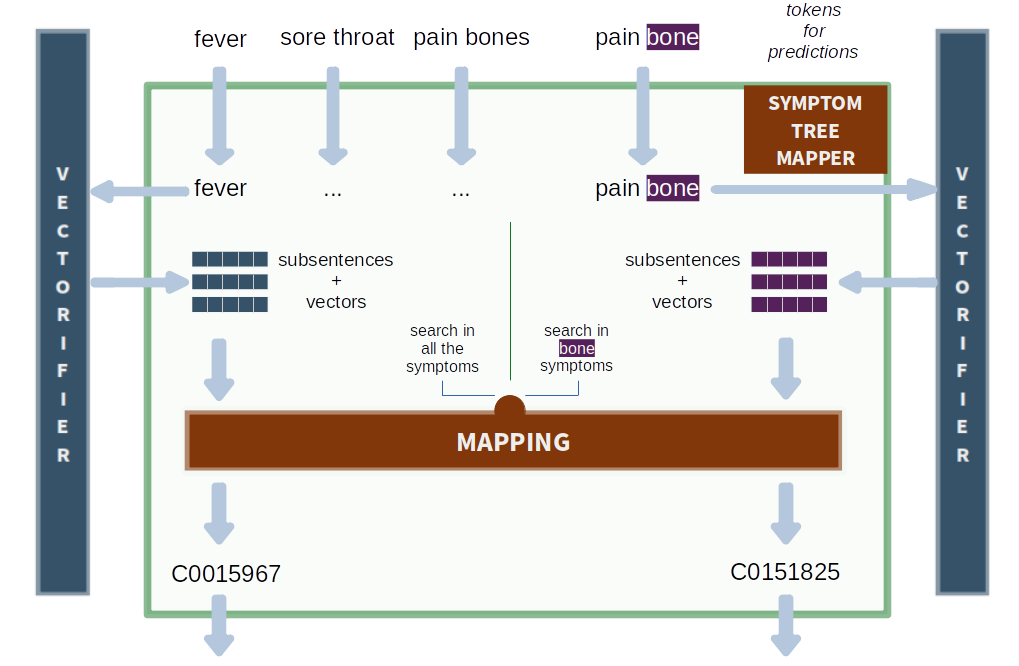
\includegraphics[width=15cm]{symptom_tree_mapper}
\caption{The Symptom Tree Mapper illustrated}
\medskip
\label{fig:symptom_t_m}
\end{figure}



\section{Symptom Tree Mapper}
\label{sec:symptom_tree_mapper}
The aim of this component is taking the \textit{tokens for predictions} (outcome of Answer Interpreter) and with the help of the Vectorifier, output the most similar symptom's CUI.

%scrivo dello stemming
In order to do this, each symptom inside the classification must have its representative vector of the same type and dimension of the embedding of the \textit{token for prediction}. Since each symptom in the classification has a descriptive field, called ``concept name'', I treated it like a sentence and I choose to use its vectorization as representative vector. In order to hasten the whole process at runtime I pre-computed these representative vectors for each supported type and dimension.

% quanti sintomi ci sono nell'albero
\subsection{The Symptom Tree}
As mentioned in section \ref{sec:cla_symp}, a suitable data structure for representing the symptom classification is a tree. In the UMLS system this hierarchy is stored with a parent array representation. The Python library that I used for this purpose is ``anytree''.

During the construction of the tree I tagged some nodes as related with a specific body part. This is helpful during mapping: given a \textit{token for prediction} that contains a body part, the search of the correct symptom is then circumscribed only to some subtrees.

\subsection{Mapping a \textit{token for prediction} to a symptom}
This phase is divided into two parts. The first consists in passing to the Vectorifier the \textit{token for prediction} and get from it the subsentences and the relative vectors; the second in computing the \textit{cosine similarity} between each subsentence vector and each symptom vector. At this point, the highest similarity shows the candidate symptom, whose CUI is predicted.

In the code there are two options that can change the process flow described above:
\begin{itemize}
  \item as mentioned earlier, if the \textit{token for prediction} contains a body part, then the mapper searches only in subtrees related to that body part (to refer to this option in the future I will use the term ``pruning'');
  \item if a \textit{minimum similarity} level is set, the prediction is output only if the highest similarity is more than this level. 
\end{itemize}



\section{How to evaluate predictions?}
\label{sec:eval_results}
Once predictions are computed, the objective is to evaluate them. This process is contextual to the sentence and it is based on a list of $m$ predictions ($[CUI_{p}1, CUI_{p}2, ..., CUI_{p}m]$) and a list of $n$ \emph{real CUIs} ($[CUI_{s}1, CUI_{s}2, ..., CUI_{s}n]$), that are the actual symptoms present in the sentence.

As mentioned in section \ref{sec:cla_symp}, the relationships between every child and every father are of type \textit{is-a}. This means that a child symptom is always a specialization of its father; in other words, the child can be viewed as a subset of its father. Thus, a prediction is considered correct if it is located within a subtree rooted in any of the real CUIs.

\begin{figure}[h]
\centering
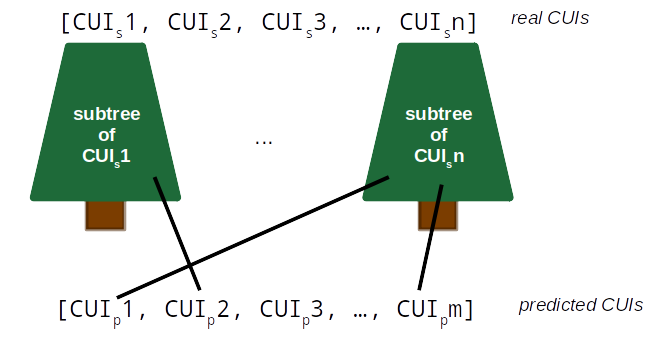
\includegraphics[width=11cm]{predictions}
\caption{Each real symptom is expanded in a subtree rooted in it. A prediction is evaluated as correct if it stays in one of these subtrees.}
\medskip
\end{figure}

\section{Dataset}
\label{sec:dataset}
%TODO prima persona
As mentioned in section \ref{datasetintro}, in order to create a suitable dataset for this project, the sentences extracted from a medical forum were linked to one or more symptoms. The used forum is \footnote{\url{https://www.doctorslounge.com/forums/}} \cite{doctorslounge} and classifies its posts by topic. The extraction and tagging process focused on six categories:
\begin{enumerate}
  \item chest
  \item ear, nose and throat
  \item eyes
  \item gastroenteric
  \item headaches
  \item pediatric 
  \item back
\end{enumerate}

Extrapolating a sentence within a post firstly means finding a passage in it which contains an identifiable and classifiable symptom and, secondly, tagging it with the relative CUI. The dataset's format is a \texttt{XML} with two types of tags: the \texttt{<sentence>} tag and the \texttt{<symptom>} tag, which has an attribute \texttt{CUI} used for linking the CUI to the symptom text.
